\documentclass[12pt,
               a4paper,
               article,
               oneside,
               oldfontcommands,
               norsk]{memoir}
\makeatletter
\newcommand*{\rom}[1]{\expandafter\@slowromancap\romannumeral #1@}
\makeatother
\usepackage[utf8]{inputenc}
\usepackage{setspace}
\usepackage[T1]{fontenc}
\usepackage{tikz}
\usepackage{lmodern}
\usepackage{enumitem}
\usepackage{caption}
\usepackage{subcaption}
\usepackage[scaled]{beramono}
\usepackage[final]{microtype}
\usepackage{amssymb}
\usepackage{mathtools}
\usepackage{amsthm}
\usepackage{thmtools}
\usepackage{babel}
\usepackage{csquotes}
\usepackage{listings}
\lstset{basicstyle = \ttfamily}
\usepackage{float}
\usepackage{textcomp}
\usepackage{siunitx}
\usepackage{xcolor}
\usepackage{graphicx}
\usepackage[colorlinks, allcolors = uiolink]{hyperref}
\pretolerance = 2000
\tolerance    = 6000
\hbadness     = 6000
\newcounter{probnum}[section]
\newcounter{subprobnum}[probnum] 
\usepackage{dirtytalk}
\usepackage{listings}
\usepackage{xcolor}
\usepackage{caption}
\usepackage[section]{placeins}
\usepackage{varwidth}
\definecolor{uiolink}{HTML}{0B5A9D}
\definecolor{codegreen}{rgb}{0,0.6,0}
\definecolor{codegray}{rgb}{0.5,0.5,0.5}
\definecolor{codepurple}{rgb}{0.58,0,0.82}
\definecolor{backcolour}{rgb}{0.95,0.95,0.92}
\lstdefinestyle{mystyle}{
    backgroundcolor=\color{backcolour},   
    commentstyle=\color{codegreen},
    keywordstyle=\color{magenta},
    numberstyle=\tiny\color{codegray},
    stringstyle=\color{codepurple},
    basicstyle=\ttfamily\footnotesize,
    breakatwhitespace=false,         
    breaklines=true,                 
    captionpos=b,                    
    keepspaces=true,                 
    numbers=left,                    
    numbersep=5pt,                  
    showspaces=false,                
    showstringspaces=false,
    showtabs=false,                  
    tabsize=3
}
\lstset{style=mystyle}
\usepackage{commath}
\usepackage{tikz}
\newtheorem{theorem}{Theorem}[section]
\newtheorem{corollary}{Corollary}[theorem]
\newtheorem{lemma}[theorem]{Lemma}


\parindent 0ex
\title{ MAT 1120\\
[0.25in]
\normalsize Obligatoriskoppgave 2}
\author{Jonas Semprini Næss}
\begin{document}
\maketitle
\section*{Oppgave 1}
\emph{Anta at $U = \left[ \boldsymbol{u}_1 \cdots \boldsymbol{u}_n \right]$ er en $n \times n$ matrise. Sjekk at $U$ er semiortogonal hvis og bare hvis $\boldsymbol{u}_j \neq \boldsymbol{0}$ for $j = 1, \hdots , n$ og $\boldsymbol{u}_j$-ene er ortogonale på hverandre, d.v.s $\boldsymbol{u}_i  \cdot \boldsymbol{u}_j= 0$ når $i \neq j$. Anta deretter at $U$ er semiortogonal og sett}
\begin{align*}
\boldsymbol{u}_{j}^{'} = \frac{1}{\boldsymbol{u}_j \cdot \boldsymbol{u}_j} \boldsymbol{u}_j,  \quad j = 1, \hdots, n
\end{align*}
\emph{Begrunn at $U$ er invertibel og at}
\begin{align*}
U^{-1} = \left[\boldsymbol{u}_{1}^{'} \cdots \boldsymbol{u}_{n}^{'}\right]^{T}.
\end{align*}
\textbf{Løsning}\vspace{3mm}\\
For å vise at $U$ er en semiortogonal matrise tar vi utgangspunkt i kravet om at $U^{T}U$ er en diagonalmatrise med kun positive koeffsienter langs hoveddiagonalen. Vi vet at 
\begin{align*}
U = \left[ \boldsymbol{u}_1 \cdots \boldsymbol{u}_n \right]
\end{align*}
hvilket gir
\begin{align*}
U^{T} = \left[ \boldsymbol{u}_1 \cdots \boldsymbol{u}_n \right]^{T} = \begin{bmatrix}
\boldsymbol{u}_1 \\
\vdots \\
\boldsymbol{u}_n
\end{bmatrix}.
\end{align*}
Videre beregner vi matriseproduktet $U^{T}U$ og sjekker om produktet oppfyller kravet.
\begin{align*}
U^{T}U &= 
\begin{bmatrix}
	\boldsymbol{u}_1 \\
	\vdots \\
	\boldsymbol{u}_n
\end{bmatrix} \left[ \boldsymbol{u}_1 \cdots \boldsymbol{u}_n \right] =
\begin{bmatrix}
	\boldsymbol{u}_1 \boldsymbol{u_1} &\cdots & \boldsymbol{u}_1 					\boldsymbol{u}_n\\
	\vdots &\ddots & \vdots \\	
	\boldsymbol{u}_n\boldsymbol{u}_1 &\cdots &\boldsymbol{u}_n\boldsymbol{u}_n
\end{bmatrix}
= \begin{bmatrix}
	\boldsymbol{u}_1 \cdot \boldsymbol{u_1} &\cdots & \boldsymbol{u}_1 	\cdot \boldsymbol{u}_n\\
	\vdots &\ddots & \vdots \\	
	\boldsymbol{u}_n \cdot \boldsymbol{u}_1 &\cdots &\boldsymbol{u}_n\cdot \boldsymbol{u}_n
\end{bmatrix}
\end{align*}
Vi husker at $\boldsymbol{u}_i  \cdot \boldsymbol{u}_j= 0$ når $i \neq j$ hvilket betyr at alle prikkprodukt i nedre og øvre del av matriseproduktet gir $0$. Videre har vi identiteten $v \cdot v = \norm{v}^{2}$, der $\norm{v}^{2} > 0$ som betyr at sluttproduktet gir en diagonal matrise (kun null entrier alle steder utenom hoveddiagonalen) med positive koeffisienter langs hoveddiagonalen, som var det vi skulle vise. \vspace{4mm}\\
Siden vektorene $\boldsymbol{u}_j,  \boldsymbol{u}_i$ for $i \neq j$ i $U$ står ortogonalt på hverandre og er forskjellig fra nullvektoren, impliserer det at vektorene er lineært uavhengige. Da følger det fra \emph{Invertibel Matrise Teoremet} at $U$ er invertibel. \vspace{4mm}\\
For å vise at $U^{-1} = \left[\boldsymbol{u}_{1}^{'} \cdots \boldsymbol{u}_{n}^{'}\right]^{T}$ skriver vi matrisen 
\begin{align*}
U^{'} = \left[\boldsymbol{u}_{1}^{'} \cdots \boldsymbol{u}_{n}^{'}\right]^{T} = \begin{bmatrix}
\boldsymbol{u}_{1}^{'}\\
\vdots \\
\boldsymbol{u}_{n}^{'}
\end{bmatrix}.
\end{align*}
Bruker vi så begrunnelsen om at $U$ er invertibel må følgende gjelde $U^{-1}U = I$ hvor $I$ er identitesmatrisen. Dermed kan vi sjekke om matriseproduktet $U^{'}U$ gir samme konklusjon. Da har vi
\begin{align*}
U^{'}U = 
\begin{bmatrix}
	\boldsymbol{u}_{1}^{'}\\
	\vdots \\
	\boldsymbol{u}_{n}^{'}
\end{bmatrix} \left[ \boldsymbol{u}_1 \cdots \boldsymbol{u}_n \right]
=
\begin{bmatrix}
	\boldsymbol{u}_{1}^{'} \boldsymbol{u}_{1} &\cdots & \boldsymbol{u}_{1}^{'} \boldsymbol{u}_n\\
	\vdots &\ddots & \vdots \\	
	\boldsymbol{u}_{n}^{'}\boldsymbol{u}_1 &\cdots &\boldsymbol{u}_{n}^{'}\boldsymbol{u}_n 
\end{bmatrix}
=
\begin{bmatrix}
	\boldsymbol{u}_{1}^{'} \cdot \boldsymbol{u}_{1} &\cdots & 							\boldsymbol{u}_{1}^{'} \cdot \boldsymbol{u}_n \\
	\vdots &\ddots & \vdots \\	
	\boldsymbol{u}_{n}^{'} \cdot \boldsymbol{u}_1 &\cdots &							\boldsymbol{u}_{n}^{'} \cdot \boldsymbol{u}_n 
\end{bmatrix}
\end{align*}
Sjekker vi for alle elementer utenfor hoveddiagonalen har vi
\begin{align*}
\frac{1}{\boldsymbol{u}_j  \cdot \boldsymbol{u}_j} \boldsymbol{u}_j \cdot \boldsymbol{u}_i = 0
\end{align*}
for $i \neq j$, og dermed er elementene langs hoveddiagonalen
\begin{align*}
\frac{1}{\boldsymbol{u}_j  \cdot \boldsymbol{u}_j} \boldsymbol{u}_j \cdot \boldsymbol{u}_i = 1
\end{align*}
for $ i = j$ hvilket betyr at vi ender opp med matrisen
\begin{align*}
\begin{bmatrix}
	1  &\cdots & 	0 \\
	\vdots &\ddots & \vdots \\	
	0 &\cdots & 1
\end{bmatrix}
\end{align*}
som er identitetsmatrisen, og vi har vist at $U^{-1} = \left[\boldsymbol{u}_{1}^{'} \cdots \boldsymbol{u}_{n}^{'}\right]^{T}$.
\section*{Oppgave 2}
\emph{Del opp $[0, \pi]$ i 3 intervaller av lengde og la $t_1, t_2, t_3$ være midtpunktene til disse intervallene:}
\begin{align*}
t_1 = \frac{\pi}{6}, \ t_2 = \frac{\pi}{2}, \ t_3 = \frac{5\pi}{6}
\end{align*}
\emph{Sett $ C_3 = \begin{bmatrix}
1 &\cos(t_1) & \cos(2t_1) \\[3pt]
1 &\cos(t_2) & \cos(2t_2) \\[3pt]
1 &\cos(t_3) & \cos(2t_3) \\[3pt]
\end{bmatrix}$, \ $S_3 = \begin{bmatrix}
\sin(t_1) &\sin(2t_1) & \sin(3t_1) \\[3pt]
\sin(t_2)&\sin(2t_2) & \sin(3t_2) \\[3pt]
\sin(t_3)&\sin(2t_3) & \sin(3t_3) \\[3pt]
\end{bmatrix}$.\vspace{2mm}\\ Regn ut $C_3$ og $S_3$ og sjekk at disse matrisene er semiortogonale. Bruk deretter Oppgave 1 til å angi
matrisene $(C_3)^{-1}$ og $(S_3)^{-1}$.}\vspace{3mm}\\
\textbf{Løsning}\vspace{3mm}\\
Setter vi inn verdiene $t_1, t_2, t_3$ i hver av matrisene får vi følgelig
\begin{align*}
C_3 = \begin{bmatrix}
1 & \frac{\sqrt{3}}{2} & \frac{1}{2} \\[4pt]
1 & 0 & -1 \\[4pt]
1 & -\frac{\sqrt{3}}{2} & \frac{1}{2}\\[4pt]
\end{bmatrix}, \quad
S_3 = \begin{bmatrix}
\frac{1}{2}& \frac{\sqrt{3}}{2} & 1 \\[4pt]
1 & 0 & -1 \\[4pt]
1 & -\frac{\sqrt{3}}{2} & 1 \\[4pt]
\end{bmatrix}
\end{align*}
Radreduserer vi hver av matrisene til redusert trappeform får vi identitetsmatrisen hvilket betyr pivoter i hver rad og kolonne (lineært uavhengige vektorer). Ser videre at alle vektorene er ulik nullvektoren ergo er matrisene semiortogonale.\vspace{3mm}\\
Ved å bruke definisjonen av den inverse matrisen til en semiortogonal kvadratisk matrise i oppgave 1.) har vi følgende ressonement.
\begin{align*}
C_{3}^{-1} = (C_{3}^{'})^{T}, \ S_{3}^{-1} = (S^{'})^{T}
\end{align*}
hvor $C_{3}^{'}, S_{3}^{'}$ er de normaliserte matrisene av $C_3, S_3$. Da har vi at
\begin{align*}
\boldsymbol{u}_1 &= \frac{1}{\boldsymbol{u}_1 \cdot \boldsymbol{u}_1} \boldsymbol{u}_1 = \frac{1}{1^2 + 1^2 + 1^2} \left(1, 1, 1 \right) \\[5pt]
\boldsymbol{u}_2 &= \frac{1}{\boldsymbol{u}_2 \cdot \boldsymbol{u}_2} = \frac{1}{\frac{3}{4} + 0 + \frac{3}{4}} \left(\frac{\sqrt{3}}{2}, 0, -\frac{\sqrt{3}}{2} \right)\\[5pt]
\boldsymbol{u}_3 &= \frac{1}{\boldsymbol{u}_3 \cdot \boldsymbol{u}_3} = \frac{1}{\frac{1}{4} + 1 + \frac{1}{4}} \left(\frac{1}{2}, -1, \frac{1}{2} \right)
\end{align*}
hvor $\boldsymbol{u}_1, \boldsymbol{u}_2, \boldsymbol{u}_3 \in C_{3}^{'}$. Det gir dermed
\begin{align*}
(C_{3}^{'})^{T} = \begin{bmatrix}
\frac{1}{3} & \frac{1}{3} & \frac{1}{3} \\[4pt]
\frac{\sqrt{3}}{3} & 0 & -\frac{\sqrt{3}}{3}\\[4pt]
\frac{1}{3} & -\frac{2}{3} & \frac{1}{3}\\[4pt]
\end{bmatrix} = C_{3}^{-1}
\end{align*} 
Følger vi samme ressonement for $S_{3}^{-1}$ gir det
\begin{align*}
(S_{3}^{'})^T = \begin{bmatrix}
\frac{1}{3} & \frac{2}{3} & \frac{1}{3} \\[4pt]
\frac{\sqrt{3}}{3} & 0 & -\frac{\sqrt{3}}{3}\\[4pt]
\frac{1}{3} & -\frac{1}{3} & \frac{1}{3}\\[4pt]
\end{bmatrix} = S_{3}^{-1}
\end{align*}
\section*{Oppgave 3}
\emph{Del opp $[0, \pi]$ i 8 intervaller av lengde $\frac{\pi}{8}$ og la $t_1, \cdots , t_8$, være midtpunktene til disse intervallene:}
\begin{align*}
t_1 = \frac{\pi}{16}, t_2 = \frac{3\pi}{16}, \cdots , \frac{15\pi}{16}
\end{align*}
\emph{m.a.o. \ $t_i = \frac{\pi}{16} + (i-1)\frac{\pi}{8}, \ i= 1,2, \ldots, 8$}\vspace{2mm}\\
\emph{La $C = \left[c_{ij} \right]$ og $S = \left[s_{ij} \right]$  være $8 \times 8$ matrisene gitt ved}
\begin{align*}
c_{ij} = \cos((j-1)t_i), \ s_{ij} = \sin(jt_i), \ i,j \in \left\{1,2 \ldots 8 \right\}
\end{align*}
\emph{Sjekk med Matlab at matrisene $C$ og $S$ er semiortogonale. Bruk deretter Oppgave 1 (og Matlab) til å beregne $C^{-1}$ og $S^{-1}$.} \vspace{3mm}\\
\textbf{Løsning}\vspace{3mm}\\
Vi kan løse oppgaven ved følgende MATLAB-script
\begin{lstlisting}[language=MATLAB]
function [C_ort, S_ort] = matrix_gen(n)
    t = zeros(n,1);
    C = zeros(n,n);
    S = zeros(n,n);
    for i = 1:n
        t(i) = pi/16 + (i-1)*pi/8;
        for j = 1:n
            C(i,j) = cos((j-1)*t(i));
            S(i,j) = sin(j*t(i));
        end
    end
   C_trans = transpose(C);
   S_trans = transpose(S);
   
   C_ort = round(mtimes(C_trans, C));
   S_ort = round(mtimes(S_trans, S));
end
\end{lstlisting}
hvilket ved gjennomkjøring gir matrisene
\begin{verbatim}
C_ort =

     8     0     0     0     0     0     0     0
     0     4     0     0     0     0     0     0
     0     0     4     0     0     0     0     0
     0     0     0     4     0     0     0     0
     0     0     0     0     4     0     0     0
     0     0     0     0     0     4     0     0
     0     0     0     0     0     0     4     0
     0     0     0     0     0     0     0     4

S_ort =

     4     0     0     0     0     0     0     0
     0     4     0     0     0     0     0     0
     0     0     4     0     0     0     0     0
     0     0     0     4     0     0     0     0
     0     0     0     0     4     0     0     0
     0     0     0     0     0     4     0     0
     0     0     0     0     0     0     4     0
     0     0     0     0     0     0     0     8
\end{verbatim}
der vi observerer at begge matrisene oppfyller kravet for å være semi-ortogonal. Utvider vi scriptet til å finne de inverse matrisene til $C$ og $S$ har vi
\begin{lstlisting}[language=MATLAB]
function [C_ort1, S_ort2, C_inv, S_inv] = matrix_gen(n)
    t = zeros(n,1);
    C = zeros(n,n);
    S = zeros(n,n);
    for i = 1:n
        t(i) = pi/16 + (i-1)*pi/8;
        for j = 1:n
            C(i,j) = cos((j-1)*t(i));
            S(i,j) = sin(j*t(i));
        end
    end
   C_trans = transpose(C);
   S_trans = transpose(S);
   
   C_ort1 = round(mtimes(C_trans, C));
   S_ort2 = round(mtimes(S_trans, S));  
   
   C_u = zeros(n);
   S_u = zeros(n);
   for k = 1:n
       cj = C(:,k);
       sj = S(:,k);
       C_u(:, k) = cj./(sum(cj.^2));
       S_u(:, k) = sj./(sum(sj.^2));
   end
   C_inv = transpose(C_u);
   S_inv = transpose(S_u); 
end
\end{lstlisting}
som gir at de inverse matrisene er
\begin{verbatim}
C_inv =

 0.125        0.125        0.125        0.125        0.125        0.125        0.125        0.125
 0.245        0.208        0.139        0.049       -0.049       -0.139       -0.208       -0.245
 0.231        0.096       -0.096       -0.231       -0.231       -0.096        0.096        0.231
 0.208       -0.049       -0.245       -0.139        0.139        0.245        0.049       -0.208
 0.177       -0.177       -0.177        0.177        0.177       -0.177       -0.177        0.177
 0.139       -0.245        0.049        0.208       -0.208       -0.049        0.245       -0.139
 0.096       -0.231        0.231       -0.096       -0.096        0.231       -0.231        0.096
 0.049       -0.139        0.208       -0.245        0.245       -0.208        0.139       -0.049


S_inv =

  0.049        0.139        0.208        0.245        0.245        0.208        0.139        0.049
  0.096        0.231        0.231        0.096       -0.096       -0.231       -0.231       -0.096
  0.139        0.245        0.049       -0.208       -0.208        0.049        0.245        0.139
  0.177        0.177       -0.177       -0.177        0.177        0.177       -0.177       -0.177
  0.208        0.049       -0.245        0.139        0.139       -0.245        0.049        0.208
  0.231       -0.096       -0.096        0.231       -0.231        0.096        0.096       -0.231
  0.245       -0.208        0.139       -0.049       -0.049        0.139       -0.208        0.245
  0.125       -0.125        0.125       -0.125        0.125       -0.125        0.125       -0.125
\end{verbatim}
\section*{Oppgave 4}
\emph{Bruk Oppgave 3 til å begrunne at $\mathcal{C}$ er en basis for $W_{c}.$ \vspace{2mm}\\Hint: Betrakt likningen}
\begin{align*}
\lambda_{1} + \lambda_{2}\cos(t) + \lambda_{3}\cos(2t) + \cdots + \lambda_{8}\cos(7t) = 0
\end{align*}
\emph{for alle $t \in [0, \pi]$, og sett inn $t = t_{1}, t_{2}, \ldots, t_{8}$.}\vspace{3mm}\\
\textbf{Løsning}\vspace{3mm}\\
Vi skriver først elementene i mengden $\mathcal{C}$ som en lineærkombinasjon av åtte vektorer.
\begin{align}
\label{eqn:vektor}
\lambda_{1} \begin{bmatrix}
1 \\[3pt]
\cos(t_{1})\\[4pt]
\vdots\\
\cos(7t_{1})
\end{bmatrix} + 
\lambda_{2} \begin{bmatrix}
1 \\[3pt]
\cos(t_{2})\\[4pt]
\vdots\\
\cos(7t_{2})
\end{bmatrix}
+
\cdots
+
\lambda_{7} \begin{bmatrix}
1 \\[3pt]
\cos(t_{7})\\[4pt]
\vdots\\
\cos(7t_{7})
\end{bmatrix}
+\lambda_{8} \begin{bmatrix}
1 \\[3pt]
\cos(t_{8})\\[4pt]
\vdots\\
\cos(7t_{8})
\end{bmatrix}
\end{align}
hvor $\lambda_{1}, \ldots, \lambda_{8} \in \mathbb{R}$ og $\left\{t_1, \ldots, t_{8} \right\} \in \left\{\frac{\pi}{16}, \ldots, \frac{15\pi}{16} \right\}$. For at en mengde vektorer skal utgjøre en basis må hver av vektorene i mengden være lineært uavhengige. Er de det er de ergo en basis for rommet de spenner ut. Dermed kan vi sette sammen vektorene i lineærkombinasjonen og radredusere den resulterende matrisen til vi (forhåptentligvis) når identitetsmatrisen. Da har vi at
\begin{align*}
A = \begin{bmatrix}
1 &\cdots & 1\\[4pt]
\cos(t_{1}) &\cdots & \cos(t_{8}) \\[4pt]
\vdots &\ddots &\vdots \\[4pt]
\cos(7t_{1}) &\cdots & \cos(7t_{8})
\end{bmatrix} = \begin{bmatrix}
1 &\cdots & 1\\[4pt]
\cos(\frac{\pi}{16}) &\cdots & \cos(\frac{15\pi}{16}) \\[4pt]
\vdots &\ddots &\vdots \\[4pt]
\cos(7\frac{\pi}{16}) &\cdots & \cos(7\frac{15\pi}{16})
\end{bmatrix} \sim \cdots \sim
\begin{bmatrix}
1  &\cdots & 0 \\[4pt]
\vdots &\ddots &\vdots \\[4pt]
0 &\cdots & 1 
\end{bmatrix}
\end{align*}
hvilket betyr at mengden $\mathcal{C}$ utgjør en basis for $W_{C}$ siden den eneste løsningen av likningsystemet \eqref{eqn:vektor} er $\lambda_{1}, \ldots, \lambda_{8} = 0$.
\section*{Oppgave 5}
\emph{Sjekk at matrisen til $T_{C}$ med hensyn på basisene $\mathcal{C}$ og $\mathcal{E}$ er matrisen $C$, og begrunn at $T_{C}$ er en isomorfi.}\vspace{3mm}\\
\textbf{Løsning}\vspace{4mm}\\
Vi har at matrisen $[T_{C}]_\mathcal{C} = \left[ T(\mathcal{C}_1) \cdots T(\mathcal{C}_8 \right]$ med hensyn på basis $\mathcal{C}$. Videre kan vi skrive matriserepresentasjonen $M$ til matrisen $T_{C}$ m.h.p basisene $\mathcal{C}$ og $\mathcal{E}$ som $M = \left[ \left[T(\mathcal{C}_1) \right]_\mathcal{E} \cdots \left[T(\mathcal{C}_8 \right]_{\mathcal{E}} \right]$. Skriver vi $M$ helt ut gir det
\begin{align*}
M &= 
	\left[ \left[T(\mathcal{C}_1) \right]_\mathcal{E} \cdots 						\left[T(\mathcal{C}_8 \right]_{\mathcal{E}} \right]\\[5pt]
&=
	\left[ \begin{bmatrix}
	\mathcal{C}_1(t_1) \\
	\vdots \\
	\mathcal{C}_1(t_8) 
	\end{bmatrix}_{\mathcal{E}} 
	\cdots
	\begin{bmatrix}
	\mathcal{C}_{8}(t_1) \\
	\vdots\\
	\mathcal{C}_8(t_8)
	\end{bmatrix}_\mathcal{E}		
	\right] \\[5pt]
&=
	\begin{bmatrix}
	1 & \cdots & \cos(7t_1) \\[3pt]
	\vdots & \ddots & \vdots \\[3pt]
	1 & \cdots & \cos(7t_8)
	\end{bmatrix}
= C
\end{align*}
hvilket vi skulle vise. Bruker vi så resultatet fra oppgave 3. husker vi at $C$ er invertibel og kan likeledes radreduseres til identitetsmatrisen. Det er ekvivalent med at det eksisterer en pivot i hver rad og kollonne hvilket betyr at $C$ er en-til-en. Da kan vi bruke Notat 2 som sier at 
\begin{itemize}
\item $T$ er en isomorfi $\iff$ $M$ er invertibel.
\item  $T$ er en isomorfi $\iff$ $T$ er $1-1$.
\end{itemize}
som stemmer i følge resultatet, og vi kan konkludere med at $T_{C}$ og $C$ er en isomorfi.
\section*{Oppgave 6}
\emph{Begrunn at $g^{C}$ er en 8-midtpunktinterpolasjon av $g$ på $[0, \pi]$, som tilfredsstiller at}
\begin{align*}
\left[g^{c} \right]_{\mathcal{C}} = C^{-1}\boldsymbol{y}
\end{align*}
\textbf{Løsning}\vspace{3mm}\\
For at en vilkårlig funksjon $k: [a,b] \rightarrow \mathbb{R}$ skal være en $n$-midtpunktinterpolasjon av en funksjon $f$ må den oppfylle kravet
\begin{align*}
k(t_1) = f(t_1), \ldots, h(t_n) = f(t_n)
\end{align*}
Her er $k = \boldsymbol{y}  = \left(g(t_1), \ldots, g(t_8) \right) \in \mathbb{R}^{8}$ og $g^{c} = T_{c}^{-1} \boldsymbol{y}$. Bruker vi opplysningen gir det
\begin{align*}
g^{c}(t_1) = g(t_1), \ldots, g^{c}(t_8) = g(t_8)
\iff
	T_{\mathcal{C}}(g^{c}) = \left( g(t_1), \ldots, g(t_8) \right) 
\end{align*}
Hvilket vi må sjekke at stemmer
\begin{align*}
T_{\mathcal{C}}(g^{c}) &= 
	T_{\mathcal{C}}\left( T_{\mathcal{C}}^{-1}(\boldsymbol{y}) 				\right) \\[5pt]
T_{\mathcal{C}}\left(T_{c}^{-1} \boldsymbol{y} \right) &=
	T_{\mathcal{C}}\left(T_{\mathcal{C}}^{-1} \left( g(t_1), \ldots, g(t_8) \right)\right)\\[5pt]
T_\mathcal{C}(g^{c}) &= (g(t_1), \ldots, g(t_8))
\end{align*}
dermed kan vi sjekke om $g^{c}$ tilfredsstiller $\left[g^{c} \right]_{\mathcal{C}} = C^{-1}\boldsymbol{y}$
\begin{align*}
\left[g^{c} \right]_{\mathcal{C}}  &= 
	\left[ T_{\mathcal{C}}^{-1}(\boldsymbol{y}) \right]_\mathcal{C} \\[5pt]
	\left[T_{c}^{-1} \boldsymbol{y}\right]_\mathcal{C} &= 							\left[T_{\mathcal{C}}^{-1} \right]_\mathcal{C}\left[\boldsymbol{y} \right]_\mathcal{E} 
=
	\left[T_{\mathcal{C}}^{-1} \right]_\mathcal{C} \boldsymbol{y} 
\end{align*}
Bruker så fra Notat 2 at $\left[T^{-1}_{\mathcal{C}} \right]_{\mathcal{C}} = \left[T_{\mathcal{C}}\right]_{\mathcal{C}}^{-1}$ og fra Oppgave 5 at $\left[T_{\mathcal{C}}\right]_{\mathcal{C}}^{-1} = C^{-1}$, slik at vi sluttvis får
\begin{align*}
\left[g^{c} \right]_{\mathcal{C}} = C^{-1}\boldsymbol{y}
\end{align*}
hvilket vi skulle vise.
\section*{Oppgave 7}
\emph{Begrunn at $V_\ell$ og $V_o$ er underrom av $V$. Sjekk deretter at hvis $f \in V$, så er $f_\ell \in V_\ell$, $f_o \in V_{o}$, og}
\begin{align*}
f = f_\ell + f_o
\end{align*}
\textbf{Løsning}\vspace{3mm}\\
For at $V_\ell$ og $V_o$ skal være underrom av $V$ må de oppfylle aksiomene
\begin{enumerate}
\item \label{itm:cond1}Nullvektoren i $V$ ligger i $V_\ell$ og $V_o$.
\item  \label{itm:cond2} $V_\ell$ og $V_o$ er lukket under addisjon.
 \item \label{itm:cond3} $V_\ell$ og $V_o$ er lukket under skalarmultiplikasjon
\end{enumerate}
Krav \ref{itm:cond1} er allerede tilfredsstilt ut i fra oppgaveteksten, som betyr at vi kan nøye oss med å vise at krav \ref{itm:cond2} og \ref{itm:cond3} også holder. For å vise \ref{itm:cond2}, \ref{itm:cond3} kan vi gjøre følgende.
\begin{align*}
(2) \ f, g &\in V_\ell \\[5pt]
h &= f + g \\[5pt]
h(-t) &= f(-t) + g(-t) \\[5pt]
h(-t) &= f(t) + g(t) \\[5pt]
h(t) &= h(t)\\[15pt]
(3) \ f &\in V_\ell \\[5pt]
	c &\in \mathbb{R}\\[5pt]
	h &= cf \\[5pt]
	h(t) &= cf(t) = cf(-t) = h(-t) \\[5pt]
	h(t) &= h(t)
\end{align*}
Tilsvarende bevis er analogt for $f(-t) = -f(t)$ (altså $V_o$), og dermed er $V_\ell$ og $V_o$ underrom av $V$. \vspace{3mm}\\
Hvis $f \in V$ så er 
\begin{align*}
f_\ell &= \frac{1}{2}\left(f + T(f) \right)\\[8pt]
f_o &= \frac{1}{2}\left(f - T(f) \right).
\end{align*}
Skal $f_\ell \in V_\ell$ og $f_o \in V_o$ må kravene $f(-t) = f(t), \ f(-t) = -f(t)$ være oppfyllt for alle $t$.
\begin{align*}
f_\ell(-t) = \frac{1}{2}\left(f + T(f) \right) =  \frac{1}{2}\left(f(t) + f(-t) \right) = f_\ell(t)
\end{align*}
tilsvarende kan vises for $f_o$. Legger vi så sammen $f_\ell$ og $f_o$ gir det 
\begin{align*}
f_\ell(t) + f_o(t) &= 
	\frac{1}{2}\left(f(t) + f(-t) \right) + \frac{1}{2}\left(f(t) - f(-t) 				\right)\\[5pt]
&=
	\frac{f(t) + f(-t) + f(t) - f(-t)}{2}\\[5pt]
&=
	\frac{2f(t)}{2} = f(t)	
\end{align*}
som var det vi ønsket å vise.
\section*{Oppgave 8}
\emph{Betrakt funksjonen}
\begin{align*}
f(t) = (\pi^2 - t^2) e^{\frac{t}{\pi}}, \ t \in [-\pi, \pi]
\end{align*}
\emph{Lag og kjør en MatLab kode som gjør følgende}
\begin{itemize}
\item Beregner vektorene $\boldsymbol{y}_\ell$ og $\boldsymbol{y}_o$
\item Beregner deretter vektorene $\boldsymbol{y}^{C}$ og $\boldsymbol{y}^{S}$ 
\item Plot grafene til $f$ og $f_{16}$ på intervallet $[-\pi, \pi]$ i samme figur.
\end{itemize}
\textbf{Løsning}\vspace{3mm}\\
Løser oppgaven ved følgende MatLab script
\begin{lstlisting}[language=MATLAB]
    n = 8;
    t = zeros(n);
    C = zeros(n,n);
    S = zeros(n,n);
    for i = 1:n
        t(i) = pi/16 + (i-1)*pi/8;
        for j = 1:n
            C(i,j) = cos((j-1)*t(i));
            S(i,j) = sin(j*t(i));
        end
    end
   C_trans = transpose(C);
   S_trans = transpose(S);
   
   C_ort1 = round(mtimes(C_trans, C));
   S_ort2 = round(mtimes(S_trans, S));  
   
   C_u = zeros(n);
   S_u = zeros(n);
   for k = 1:n
       cj = C(:,k);
       sj = S(:,k);
       C_u(:, k) = cj./(sum(cj.^2));
       S_u(:, k) = sj./(sum(sj.^2));
   end
   C_inv = transpose(C_u);
   S_inv = transpose(S_u);
   
   t_16 = linspace(pi/16, 15*pi/16, 8);
   t = linspace(-pi, pi, 10000);
   
   f_t16 = (pi.^2. - (t_16.^2)).*exp(t_16./pi);
   f_t16_n = ((pi.^2.- ((-t_16).^2)).*exp((-t_16)./pi));
   
   f_l = 0.5*(f_t16 + f_t16_n);
   f_o = 0.5*(f_t16 - f_t16_n);
   
   y_c = mtimes(C_inv, transpose(f_l));
   y_s = mtimes(S_inv, transpose(f_o));
   
   f_16 = y_c(1) + y_c(2)*cos(t) + y_c(3)*cos(2*t) + y_c(4)*cos(3*t) ...
     + y_c(5)*cos(4*t) + y_c(6)*cos(5*t) + y_c(7)*cos(6*t)... 
     + y_c(8)*cos(7*t)+ y_s(1)*sin(t) + y_s(2)*sin(2*t)... 
     + y_s(3)*sin(3*t) + y_s(4)*sin(4*t)+ y_s(5)*sin(5*t)...  
     + y_s(6)*sin(6*t)  + y_s(7)*sin(7*t) + y_s(8)*sin(8*t);
     
     
   f = (pi.^2 - t.^2).*exp(t./pi);
   g = figure;
   plot(t, f, ' r ' , t , f_16 , 'b')
   ax = gca;
   ax.FontSize = 15;
   xlabel('x');
   ylabel('y');
   title('Plot av f og f_{16},  f = \pi^2 - t^2 \cdot e^{(t/pi)}');
   saveas(g,'oppgave_8', 'png')
\end{lstlisting}
som gir følgende plot.
\begin{figure}[H]
	\centering
	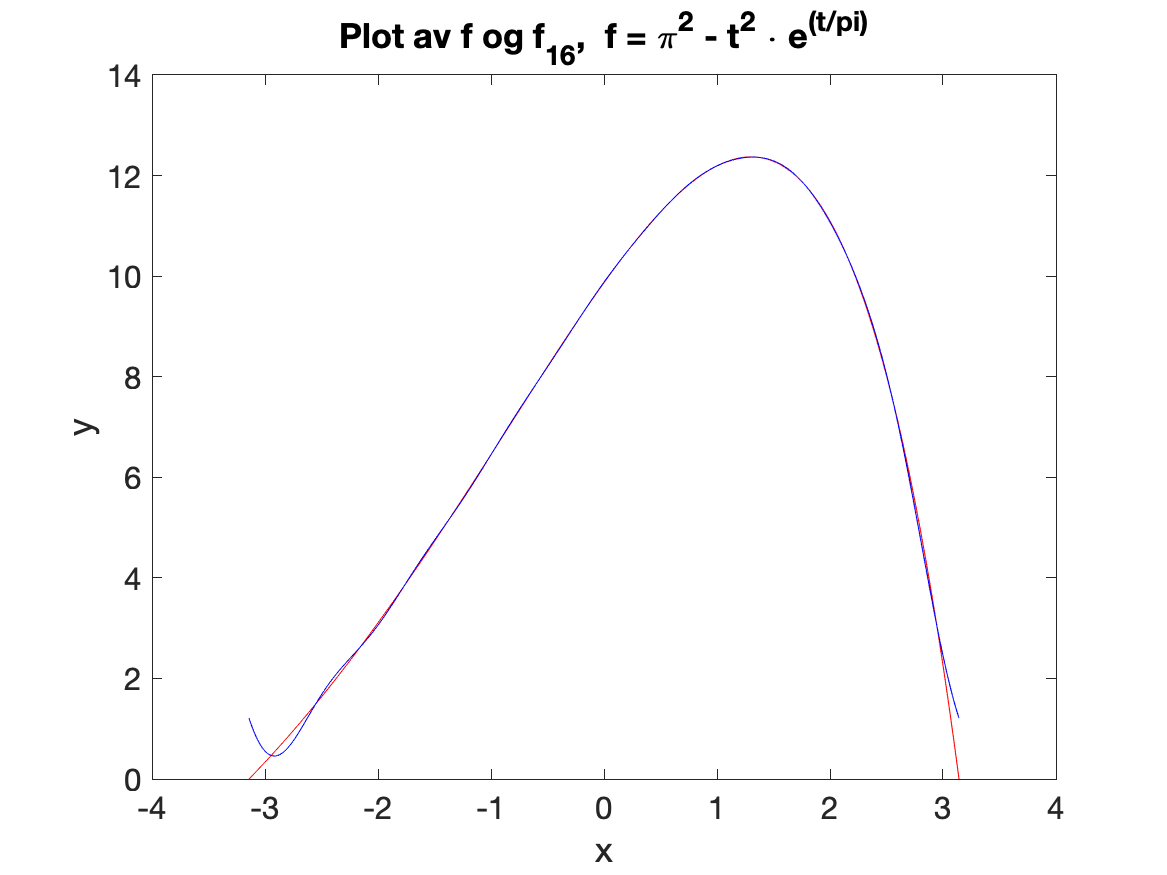
\includegraphics[scale=0.7]{oppgave_8.png} 
\end{figure}
\section*{Oppgave 9}
\emph{Gjenta punktene i Oppgave 8 med funksjonen $f(t)= 1/(1 + 4t^2)$, og deretter funksjonen $f(t) = \tan(t/4)$ (der $t \in [-\pi, pi]$ i begge tilfellene).}\vspace{3mm}\\
\textbf{Løsning}\vspace{3mm}\\
Modifiserer vi scriptet i Oppgave 8. med opplysningene i oppgaven får vi følgende to kildekoder
\begin{lstlisting}[language=MATLAB]
	 n = 8;
    t = zeros(n);
    C = zeros(n,n);
    S = zeros(n,n);
    for i = 1:n
        t(i) = pi/16 + (i-1)*pi/8;
        for j = 1:n
            C(i,j) = cos((j-1)*t(i));
            S(i,j) = sin(j*t(i));
        end
    end
   C_trans = transpose(C);
   S_trans = transpose(S);
   
   C_ort1 = round(mtimes(C_trans, C));
   S_ort2 = round(mtimes(S_trans, S));  
   
   C_u = zeros(n);
   S_u = zeros(n);
   for k = 1:n
       cj = C(:,k);
       sj = S(:,k);
       C_u(:, k) = cj./(sum(cj.^2));
       S_u(:, k) = sj./(sum(sj.^2));
   end
   C_inv = transpose(C_u);
   S_inv = transpose(S_u);
   
   t_16 = linspace(pi/16, 15*pi/16, 8);
   t = linspace(-pi, pi, 10000);
   
   f_t16 = 1./(1 + 4.*t_16.^2);
   f_t16_n = 1./(1 + 4.*(-t_16).^2);
   
   f_l = 0.5*(f_t16 + f_t16_n);
   f_o = 0.5*(f_t16 - f_t16_n);
   
   y_c = mtimes(C_inv, transpose(f_l));
   y_s = mtimes(S_inv, transpose(f_o));
   
   f_16 = y_c(1) + y_c(2)*cos(t) + y_c(3)*cos(2*t) + y_c(4)*cos(3*t)... 
    + y_c(5)*cos(4*t) + y_c(6)*cos(5*t) + y_c(7)*cos(6*t)... 
    + y_c(8)*cos(7*t) + y_s(1)*sin(t) + y_s(2)*sin(2*t) ...
    + y_s(3)*sin(3*t)  + y_s(4)*sin(4*t)  + y_s(5)*sin(5*t)... 
    + y_s(6)*sin(6*t)  + y_s(7)*sin(7*t) + y_s(8)*sin(8*t);

   f = 1./(1 + 4.*t.^2);
   g = figure;
   plot(t, f, ' r ' , t , f_16 , 'b')
   ax = gca;
   ax.FontSize = 15;
   xlabel('x');
   ylabel('y');
   title('Plot av f og f_{16},  f = 1/(1 + 4t^2)');
   saveas(g,'oppgave_9', 'png'
\end{lstlisting}
\begin{lstlisting}[language=MATLAB]
    n = 8;
    t = zeros(n);
    C = zeros(n,n);
    S = zeros(n,n);
    for i = 1:n
        t(i) = pi/16 + (i-1)*pi/8;
        for j = 1:n
            C(i,j) = cos((j-1)*t(i));
            S(i,j) = sin(j*t(i));
        end
    end
   C_trans = transpose(C);
   S_trans = transpose(S);
   
   C_ort1 = round(mtimes(C_trans, C));
   S_ort2 = round(mtimes(S_trans, S));  
   
   C_u = zeros(n);
   S_u = zeros(n);
   for k = 1:n
       cj = C(:,k);
       sj = S(:,k);
       C_u(:, k) = cj./(sum(cj.^2));
       S_u(:, k) = sj./(sum(sj.^2));
   end
   C_inv = transpose(C_u);
   S_inv = transpose(S_u);
   
   t_16 = linspace(pi/16, 15*pi/16, 8);
   t = linspace(-pi, pi, 10000);
   
   f_t16 = tan(t_16./4);
   f_t16_n = tan(-t_16./4);
   
   f_l = 0.5*(f_t16 + f_t16_n);
   f_o = 0.5*(f_t16 - f_t16_n);
   
   y_c = mtimes(C_inv, transpose(f_l));
   y_s = mtimes(S_inv, transpose(f_o));
   
   f_16 = y_c(1) + y_c(2)*cos(t) + y_c(3)*cos(2*t) + y_c(4)*cos(3*t)... 
   + y_c(5)*cos(4*t) + y_c(6)*cos(5*t) + y_c(7)*cos(6*t)... 
   + y_c(8)*cos(7*t) + y_s(1)*sin(t) + y_s(2)*sin(2*t)... 
   + y_s(3)*sin(3*t)  + y_s(4)*sin(4*t)  + y_s(5)*sin(5*t)...  
   + y_s(6)*sin(6*t)  + y_s(7)*sin(7*t) + y_s(8)*sin(8*t);

   f = tan(t./4);
   g = figure;
   plot(t, f, ' r ' , t , f_16 , 'b')
   ax = gca;
   ax.FontSize = 15;
   xlabel('x');
   ylabel('y');
   title('Plot av f og f_{16},  f = tan(t/4)');
   saveas(g,'oppgave_9_b', 'png')
\end{lstlisting}
som sluttvis gir plottene
\begin{figure}[H]
	\centering
	\begin{subfigure}[H]{0.8\textwidth}
	\centering
	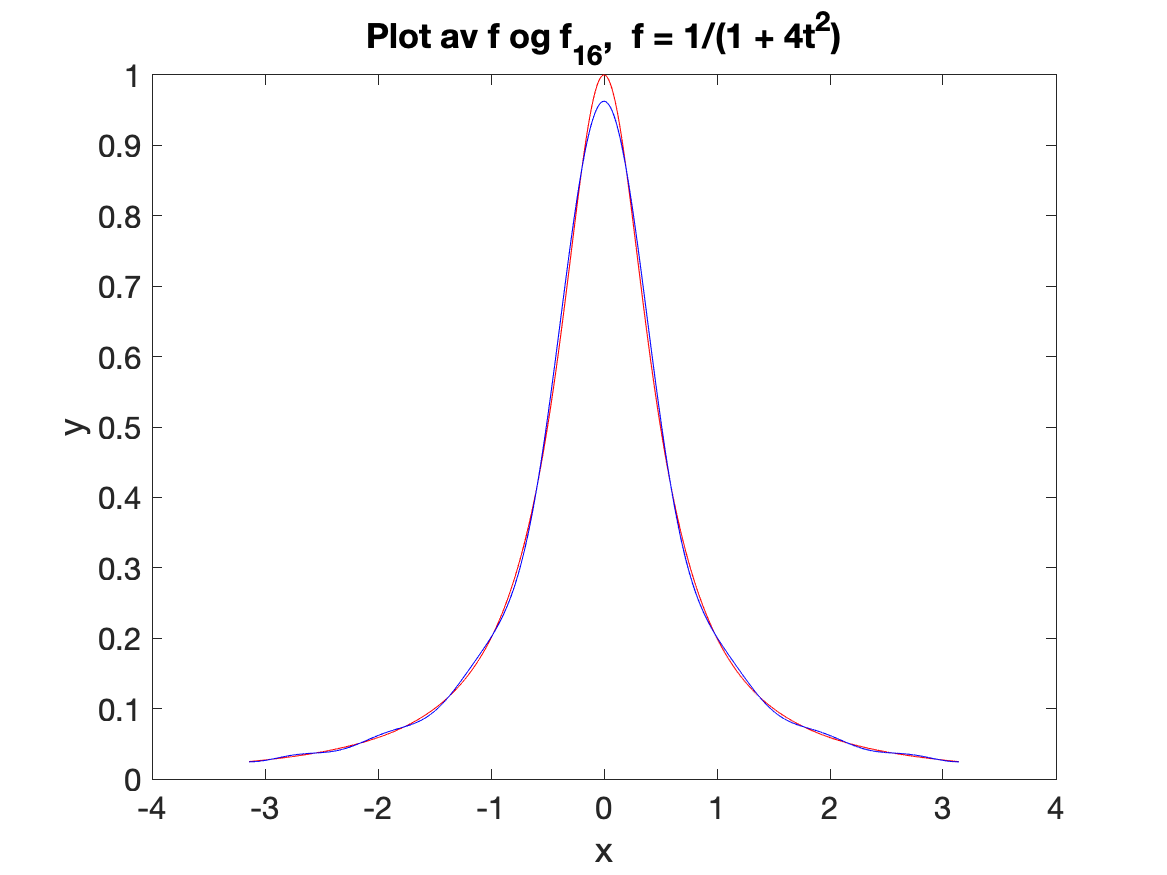
\includegraphics[width=\textwidth]{oppgave_9.png}
	\end{subfigure}
	\vfill
	\begin{subfigure}[H]{0.8\textwidth}
	\centering
	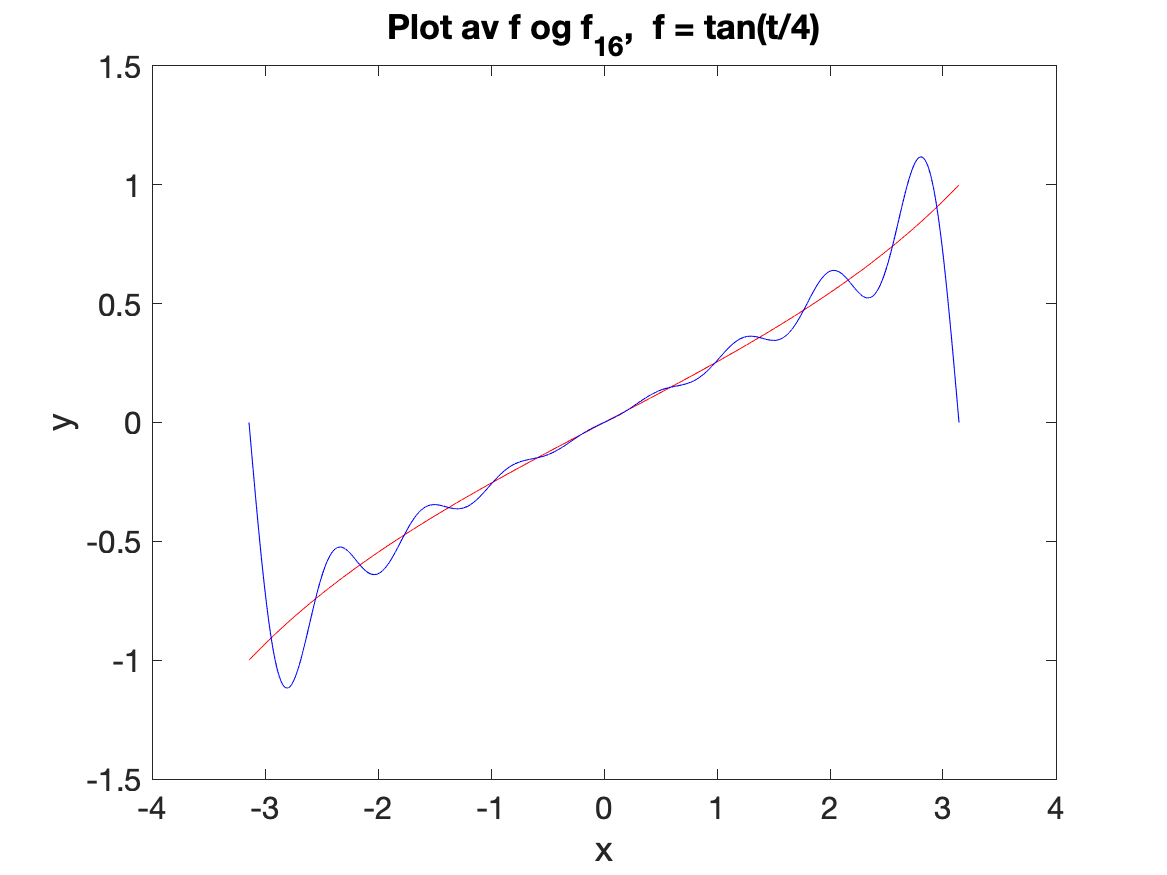
\includegraphics[width=\textwidth]{oppgave_9_b.png} 
	\end{subfigure}
\end{figure}
\end{document}